% !TEX encoding = UTF-8 Unicode
\RequirePackage{fix-cm}
\documentclass[a4paper,10pt,UTF8]{paper}
%\documentclass[a4paper,10pt,UTF8]{ctexart}

\usepackage[english]{babel}
\usepackage{fancyhdr,array,lastpage,amsmath,mathtools,enumitem,graphicx,multirow,tocbibind,longtable,makecell,varwidth,titlesec,bm,booktabs,comment,minted}
\usepackage{enumitem}
\usepackage{hyperref}
\hypersetup{hidelinks}
%\setCJKmainfont[BoldFont=Heiti SC Medium]{Songti SC Light}
%\setCJKsansfont{Heiti SC}

\usepackage[left=2.54cm,right=2.54cm,top=2.54cm,bottom=2.54cm]{geometry}
\usepackage[font=footnotesize,labelfont=bf]{caption}
\usepackage{tikz,flowchart}
\usepackage{ctex}
\usetikzlibrary{shapes,shapes.geometric,arrows,matrix,calc}
\usetikzlibrary{circuits.logic}
% \usetikzlibrary{circuits.logic.custom}
\usetikzlibrary{circuits.logic.IEC}
\usetikzlibrary{shadows}
\usepackage{listings}
\usepackage[Q=yes]{examplep}
\usepackage{fancyhdr}
\usepackage{alphalph}
\usepackage{indentfirst}

\newenvironment{sol}
  {\par\vspace{2mm}\noindent{\bf Solution}. }

\lstset{escapeinside=``, breaklines=true, frame=none, extendedchars=false, basicstyle=\ttfamily, showstringspaces=false}


\setlength{\parindent}{2em}
\setlength{\parskip}{1.5ex plus 0.5ex minus 0.2ex}
\linespread{1.1}

\bibliographystyle{plain}

\numberwithin{equation}{section}
\numberwithin{figure}{section}

\usepackage{karnaugh}
\usepackage{circuitikz}


\setcounter{secnumdepth}{3}
\setcounter{tocdepth}{3}

\title{华东师范大学计算机科学技术系上机实验报告}

\begin{document}
\pagestyle{fancy}
\chead{\small\color{gray}华东师范大学计算机科学技术系上机实验报告}
\lhead{}
\rhead{}
\makeatletter
\def\headrule{{\if@fancyplain\let\headrulewidth\plainheadrulewidth\fi%
\color{gray}\hrule\@height 0.2pt\@width\headwidth}
  \vspace{6mm}}
\makeatother

\newcommand{\HRule}{\rule{\linewidth}{1mm}}
\newcommand{\dai}{\textbf{Dais-CMX16$^+$}}

{\center {\huge \bfseries \LARGE{华东师范大学计算机科学技术系上机实验报告}} \\ [0.8cm]

\small{
  \begin{minipage}[t]{.32\linewidth}
    \textbf{课程名称:}计算机组成与结构实践\\
    \textbf{指导教师:}金健\\
    \textbf{上机实践名称:} TODO\\
    \textbf{实践编号:}实验 1
  \end{minipage}
  \begin{minipage}[t]{.32\linewidth}
    \textbf{年级:}17 级\\
    \textbf{姓名:}朱桐\\
    \textbf{学号:}10175102111\\
    \textbf{组号:}A
  \end{minipage} 
  \begin{minipage}[t]{.32\linewidth}
    \textbf{上机实践成绩:} \\
    \textbf{创新实践成绩:} \\
    \textbf{上机实践日期:}2019/09/20\\
    \textbf{上机实践时间:}2 学时\\
  \end{minipage}
}
\HRule \\[0.5cm]
}
\section{实验目的}

熟悉Keil中的汇编语言格式,并能熟练运用存储器访问指令、通用数据处理指令、分支指令(LDR、STR、CMP、B、AND等)编写简单的汇编程序;


\section{实验设备}

熟悉Keil中的汇编语言格式,并能熟练运用存储器访问指令、通用数据处理指令、分支指令(LDR、STR、CMP、B、AND等)编写简单的汇编程序;

\section{实验内容}
\begin{itemize}
  \item 学习示例汇编代码,根据题目编写ARM汇编程序
  \item 单步调试,观察寄存器值、内存的变化情况以及执行结果
  \item 练习1:模仿上面的例子程序,统计自己学号中奇数数字的个数,学号以ASCII的形式存储并以\#号作为结束符,字符以字节为单位存储。(关于ASCII表,'0'对应(0x30),'9'对应(0x39),'\#'对应(0x23))
  \item 练习2: 给定一个数组(数组大小为5,例如5,4,3,2,1),对该数组进行升序排序。
\end{itemize}


\section{实验原理}

\subsection{ARM汇编中各个寄存器简介
}

\begin{itemize}
  \item R0-R7:低位寄存器,指定通用寄存器的所有指令均可访问R0-R7。
  \item R8-R12:高位寄存器,指定通用寄存器的所有32位指令均可访问R8-R12。并非所有16位指令都可以访问寄存器R8-R12。
  \item 寄存器R13用作堆栈指针(SP)。
  \item 寄存器R14是子程序链接寄存器(LR)。当执行分支指令(BL、BLX)时,LR从PC接收返回地址。另外,LR也可用于异常返回。在其他情况下,可以将R14作为通用寄存器使用。
  \item 寄存器R15是程序计数器(PC)。
  \item xPSR(程序状态寄存器)在内部可分为3个子状态寄存器:应用程序状态寄存器(APSR)、中断程序状态寄存器(IPSR)和执行程序状态寄存器(EPSR)。通过MRS/MSR指令,这3个PSR可以单独访问,也可组合访问。

\end{itemize}


限定某种条件才能执行指令,如跳转指令B, BEQ为等于时跳转,BNE为不等于时跳转,条件码表如下 \ref{fig:1}

\begin{figure}[h]
  \centering
  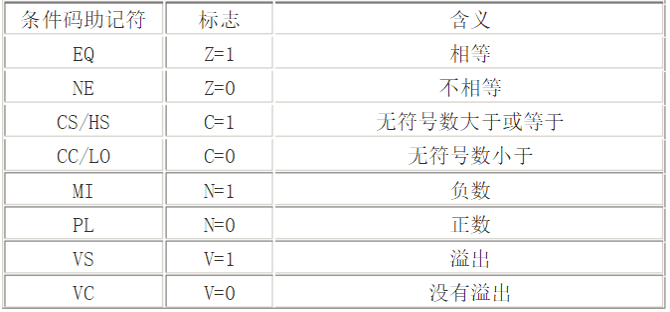
\includegraphics[width=0.9\textwidth]{1.PNG}
  \caption{条件码}
  \label{fig:1}
\end{figure}


\section{实验步骤}

\subsection{练习1}

仿照样例程序,我们只接受asc码大于等于 0x30 和 0x39 之间的字符,然后减去 0x30 得到实际的数字,和上一次的实验一样使用 TST 和 ADDNE 后缀完成任务

\subsection{练习2}

先把常量数组拷贝到 sram(0x20000000) 中,然后再使用冒泡排序,对应的 c++ 语言程序如下

\begin{minted}[mathescape,
  linenos,
  numbersep=5pt,
  gobble=2,
  frame=lines,
  framesep=2mm]{cpp}
  void sort(vector<int> &a) {
    int n = a.size();
    for (int i=0; i<n-1; ++i) {
        for (int j=n-1; j>i; --j) {
            if (a[j] < a[j-1]) swap(a[j], a[j-1]);
        }
    }
  }
\end{minted}

之后我们可以翻译程序了,使用 MOV 完成赋值,swap语句;使用 BNE(BGT,BLT) 完成for循环语句

\section{调试过程、结果与分析}



\section{总结}

\section{附件}

\end{document}
